\documentclass{article}
\usepackage[utf8]{inputenc}
\usepackage{amssymb}
\usepackage{graphicx}
\usepackage{tikz}
\usepackage[margin=1in]{geometry}
\usepackage[absolute,overlay]{textpos}
\usepackage{graphicx}


\title{Eigenvalue collisions for
matrix processes associated with Ginibre matrices}
\author{Carlos Vargas}
\date{\today}

\begin{document}
	\maketitle	
	\begin{abstract}
	Bla
 	\end{abstract} 

	\section{Introduction}
	We study the collisions of eigenvalues for a family of matrices 
	$$R(s,t) = \alpha(s)C + \beta(s)U(t),$$ 
	periodic on the parameter $t\in [0,1]$, with $s\in [0, 1]$,   
	determined by a realization of a Ginibre matrix $C \in M_N(\mathbb{C})$ 
	and a periodic matrix $U(t)$, 
	with equidistant points along the unit circle, 
	or some other curve. 
		
	Roughly speaking, in order to search for eigenvalue collisions, 
	we fix $s$, and slowly increase the periodic value $t$, 
	while keeping track of all eigenvalues.	
	
	Unless $s$ is too close to $0$ or fairly close to $1$, 
	the process of increasing $t$ leads in general to a non-trivial permutation $\sigma(s)$, 
	with pleasing visualizations of flowing, repellent eigenvalues, 
	that proceed to team-up and whirl, as $s$ increases,
	first around themselves and then around zero.
	
	The intricate web of paths that the eigenvalues collectively traverse 
	remains quite stable for small variations in $s$. 
	However, the actual permutations $\sigma(s)$, $\sigma(s + \Delta s)$ 
	may present variations, 
	indicating eigenvalue collisions 
	at some intermediate values $(s,t)$, $s\in (s, s + \Delta s)$,
	which explain the permutation discrepancy.	
	These collisions are also indicative of local maxima for the speed of eigenvalues 
	and for the variation on their tracks.

	We report some first statistics about these processes and their collisions, 
	and we include a simple package to perform/store/display these (parallellizable) 
	computations.

	\subsection{Ginibre Matrix}

	\begin{figure}[htbp]
    \centering
    % Row 1
    \begin{minipage}[b]{0.48\textwidth}
        \centering
        \includegraphics[width=\textwidth]{/home/charli/Math/eigenvalueCollissions/animatedGinibre/plot_1.pdf}
    \end{minipage}
    \hfill
    \begin{minipage}[b]{0.48\textwidth}
        \centering
        \includegraphics[width=\textwidth]{/home/charli/Math/eigenvalueCollissions/animatedGinibre/plot_2.pdf}
    \end{minipage}

    % Row 2
    \vspace{0.5cm}
    \begin{minipage}[b]{0.48\textwidth}
        \centering
        \includegraphics[width=\textwidth]{/home/charli/Math/eigenvalueCollissions/animatedGinibre/plot_3.pdf}
    \end{minipage}
    \hfill
    \begin{minipage}[b]{0.48\textwidth}
        \centering
        \includegraphics[width=\textwidth]{/home/charli/Math/eigenvalueCollissions/animatedGinibre/plot_4.pdf}
    \end{minipage}

    % Row 3
    \vspace{0.5cm}
    \begin{minipage}[b]{0.48\textwidth}
        \centering
        \includegraphics[width=\textwidth]{/home/charli/Math/eigenvalueCollissions/animatedGinibre/plot_5.pdf}
    \end{minipage}
    \hfill
    \begin{minipage}[b]{0.48\textwidth}
        \centering
        \includegraphics[width=\textwidth]{/home/charli/Math/eigenvalueCollissions/animatedGinibre/plot_6.pdf}
    \end{minipage}
    
    \caption{Comparison of different eigenvalue visualizations.}
    \label{fig:comparison}
	\end{figure}

	A Ginibre matrix is just a square $N\times N$ random matrix, 
	consisting of independent, identically distributed entries 
	with zero-mean and the same finite variance $\sigma$. 
	
	The well known "Circular law" states that if $\sigma = 1/N$ the 
	empirical distribution of the eigenvalues converges almost surely,
	as $N\to \infty$, to the uniform distribution on the centered unit disc.
	
	Similar to the central limit theorem, 
	the circular law is universal: 
	it holds for matrices with independent entries 
	following any centered, finite variance distribution,
	such as the complex gaussian, 
	real gaussian, or symmetric bernoulli distributions (see Figure).
	
	We notice in the figures that the two real-valued matrices have conjugated eigenvalues
	(as any real-valued matrices do),  
	but otherwise the distributions look fairly similar and quite regularly covering the unit disk.

	For the complex gaussian case, the explicit joint density function for
	the eigenvalues is:

	$$\rho (\lambda_1, \dots , \lambda_N) = 
	\frac{1}{\pi^n \prod_{k=1}^N k!}
	\exp(-\sum_{k=1}^N |\lambda_{k}|^{-2}) 
	\prod_{1\leq j < k \leq N} |\lambda_k - \lambda_j|^2$$

	The eigenvalues of Ginibre matrices repell each other. 
	This leads to more uniform patterns of eigenvalues and faster/stronger convergence results 
	to the limit asymptotic distributions 
	(compare $400$ eigenvalues with $400$ independent points in the disc).  

	\subsection{Model description}

	Consider a realization $C \in M_N(\mathbb{C})$ of an $N\times N$ Ginibre matrix and 
	let $\omega$ be the first clock-wise non-trivial complex $N$-th root of $1$. 
	For $t\in [0,1]$ let
	$$U(t) = \mathrm{diag}(\omega^{tN}, \omega^{tN+1}, \omega^{tN+2}, \dots   , \omega^{tN+N-1}),$$ 
	be a diagonal matrix with equi-distant points along the circle. Notice that $U(0) = U(1)$.

	We want to study the eigenvalues of the matrix model:
	$$R(s,t) = \alpha(s)C + \beta(s)U(t),\quad  \alpha(s)= \cos((s\pi)/2),\quad \beta(s)= \sin((s\pi) /2),$$ 
	which is periodic on $t\in [0,1]$ for a fixed $s$.

	In general it is quite a task to compute distributions 
	of non-selfadjoint random matrix models. 
	The matrices in this model, however, 
	are approximations of R-diagonal elements in free probability, 
	for which some actual computations for asymptotic distributions have been made [?,?]. 

	Depending on the values of $\alpha$ and $\beta$, 
	the asymptotic distribution (as $N\to\infty$) is supported on a centered annulus or a disk, 
	more dense on the outer side. 
	(see Figure). 
	
	\begin{figure}[htbp]
		\centering
		% Row 1
		\begin{minipage}[b]{0.48\textwidth}
			\centering
			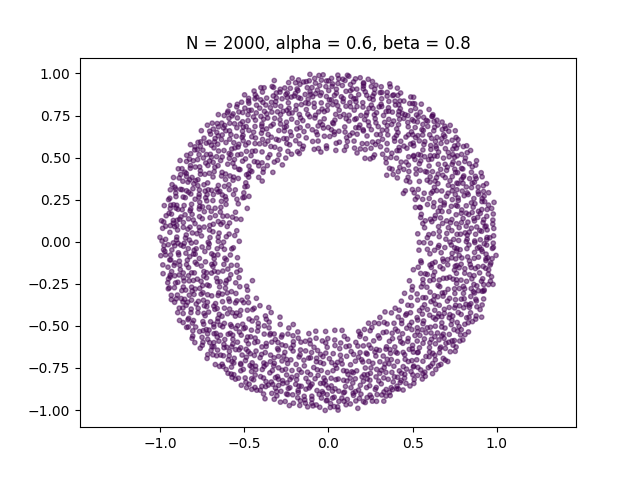
\includegraphics[width=\textwidth]{/home/charli/Math/eigenvalueTracking/animatedGinibre/Figure_1.png}
			\caption{Figure 1 description.}
		\end{minipage}
		\hfill
		\begin{minipage}[b]{0.48\textwidth}
			\centering
			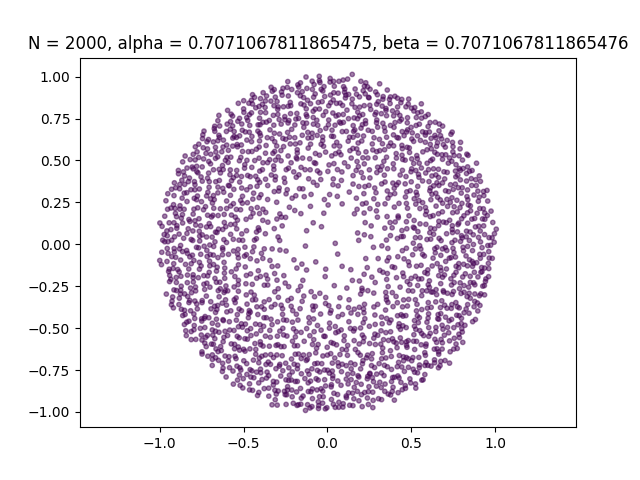
\includegraphics[width=\textwidth]{/home/charli/Math/eigenvalueTracking/animatedGinibre/Figure_2.png}
			\caption{Figure 2 description.}
		\end{minipage}
	
		% Row 2
		\vspace{0.5cm}
		\begin{minipage}[b]{0.48\textwidth}
			\centering
			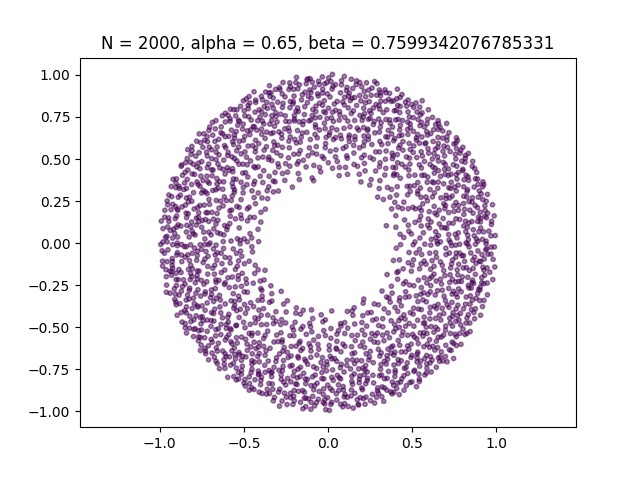
\includegraphics[width=\textwidth]{/home/charli/Math/eigenvalueTracking/animatedGinibre/Figure_3.png}
			\caption{Figure 3 description.}
		\end{minipage}
		\hfill
		\begin{minipage}[b]{0.48\textwidth}
			\centering
			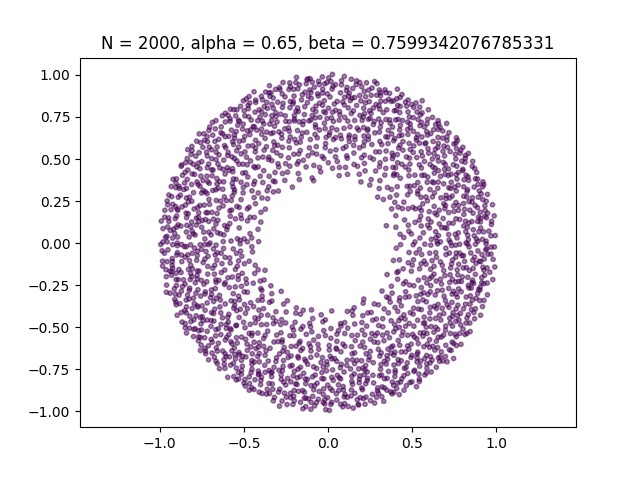
\includegraphics[width=\textwidth]{/home/charli/Math/eigenvalueTracking/animatedGinibre/Figure_3.png}
			\caption{Figure 4 description.}
		\end{minipage}
	
		\caption{Comparison of eigenvalue tracking results.}
		\label{fig:comparison_2x2}
	\end{figure}
	

	We choose $\alpha(s) = \cos(s \pi /2)$ and $\beta(s) = \sin(s \pi /2)$ 
	specificaly to keep the outer radious of the model approximately equal to one. 
	The eigenvalues for any other positive pairs $(\alpha, \beta)$ can be obtained 
	by properly scaling values within this parametrization.
	
	In this work we mainly want to draw attention at the effect of increasing 
	the periodic parameter $t$,
	which 'turns' the eigenvalues of the model clockwise.

	The figures show one set of eigenvalues (red circles) 
	trailing the next set of eigenvalues 
 	after small increases of t (blue stars)

	 \begin{figure}[htbp]
		\centering
		% Row 1
		\begin{minipage}[b]{0.48\textwidth}
			\centering
			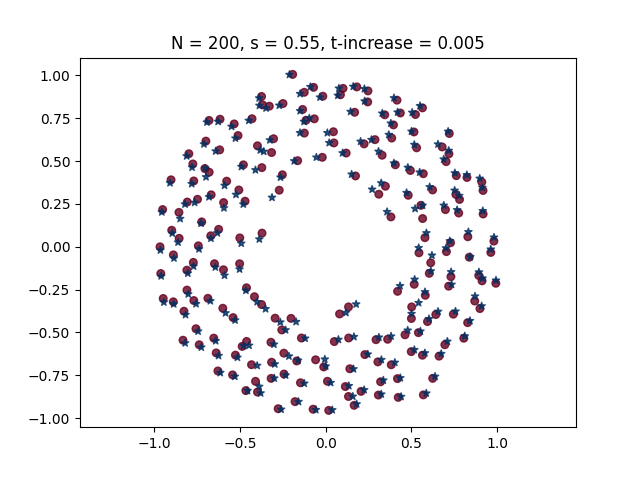
\includegraphics[width=\textwidth]{/home/charli/Math/eigenvalueTracking/animatedGinibre/Figure_10.png} 
			\caption{Figure 1 description.}
		\end{minipage}
		\hfill
		\begin{minipage}[b]{0.48\textwidth}
			\centering
			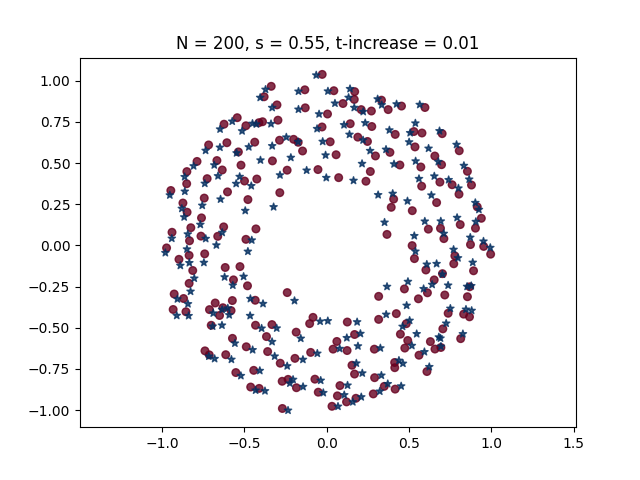
\includegraphics[width=\textwidth]{/home/charli/Math/eigenvalueTracking/animatedGinibre/Figure_8.png} 
			\caption{Figure 2 description.}
		\end{minipage}
	
		% Row 2
		\vspace{0.5cm}
		\begin{minipage}[b]{0.48\textwidth}
			\centering
			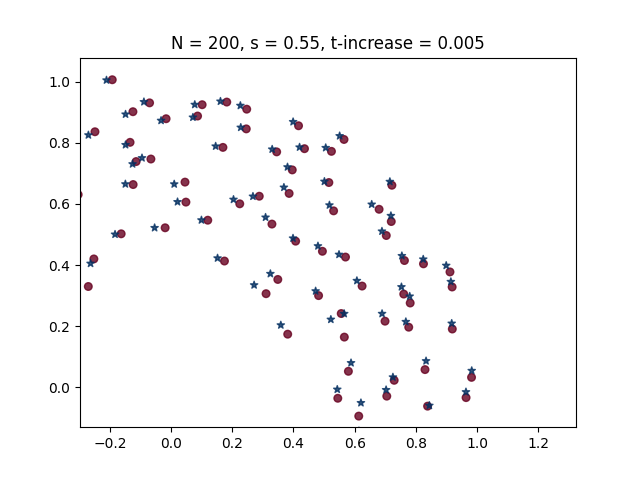
\includegraphics[width=\textwidth]{/home/charli/Math/eigenvalueTracking/animatedGinibre/Figure_11.png} 
			\caption{Figure 3 description.}
		\end{minipage}
		\hfill
		\begin{minipage}[b]{0.48\textwidth}
			\centering
			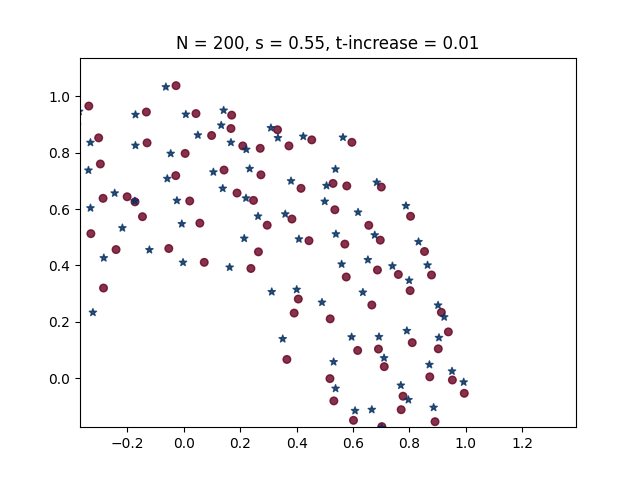
\includegraphics[width=\textwidth]{/home/charli/Math/eigenvalueTracking/animatedGinibre/Figure_9.png}
			\caption{Figure 4 description.}
		\end{minipage}
	
		\caption{Comparison of eigenvalue tracking results.}
		\label{fig:comparison_2x2}
	\end{figure}

	Notice that the eigenvalues in the outer part of the domain are moving much more slowly 
	than the eigenvalues on the inner part.

	On the other hand, since $U(0) = U(1)$, as $t$ increases from zero to one, 
	most eigenvalues won't make a complete turn to return to their original positions, 
	but each eigenvalue must return to \emph{some other eigenvalues's original position}, as $t$ reaches $1$. 

	This leads to a non-trivial permutation $\sigma(s)$ 
	associated with the matrix process at the value $s$.

	The model makes sense if we replace the  unit circle by any parametrized curve... 
	(TODO: Use the same (star, circle) format. Same N, circuit and crossing ... )

	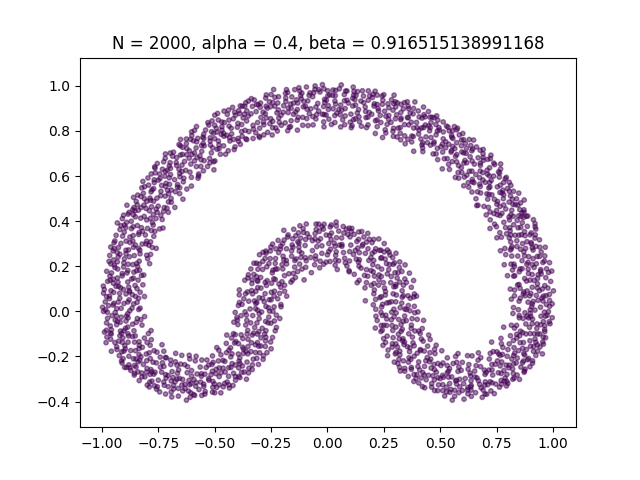
\includegraphics[width=0.5\textwidth]{/home/charli/Math/eigenvalueTracking/animatedGinibre/Figure_5.png} 
	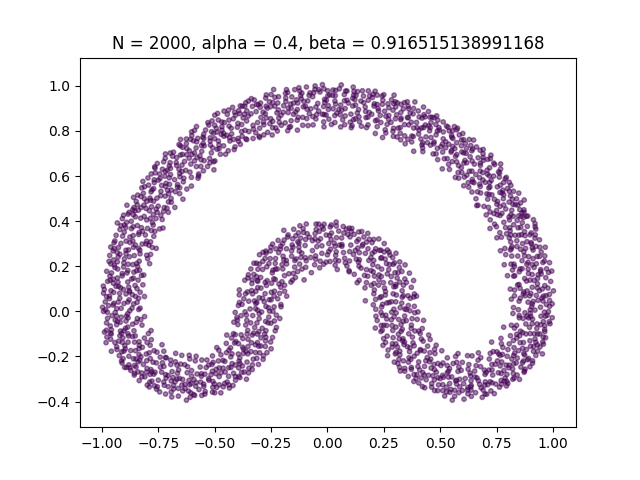
\includegraphics[width=0.5\textwidth]{/home/charli/Math/eigenvalueTracking/animatedGinibre/Figure_5.png} 
	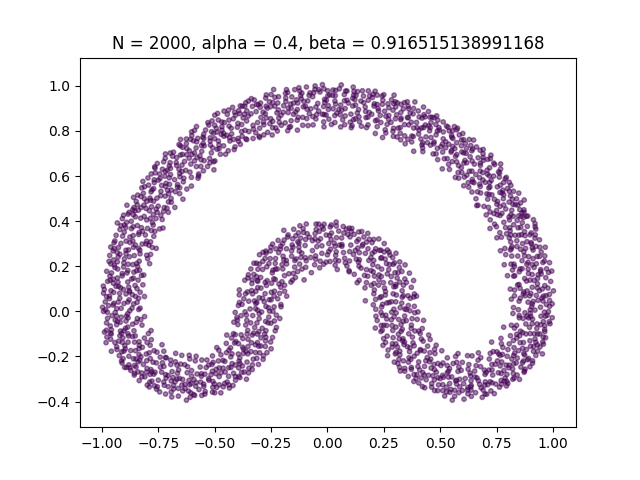
\includegraphics[width=0.5\textwidth]{/home/charli/Math/eigenvalueTracking/animatedGinibre/Figure_5.png} 
	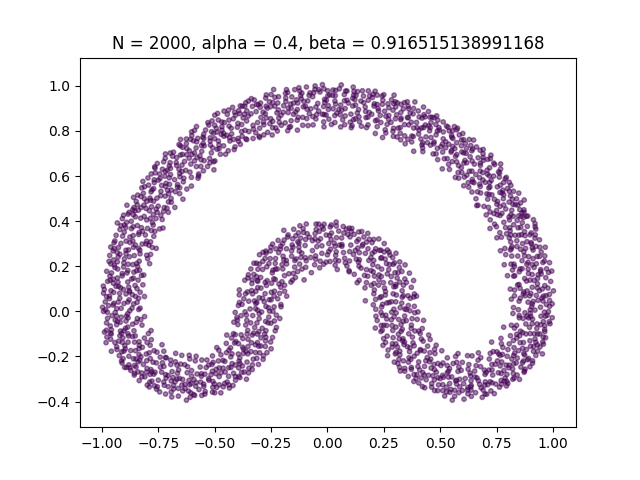
\includegraphics[width=0.5\textwidth]{/home/charli/Math/eigenvalueTracking/animatedGinibre/Figure_5.png}
	
	We use the permutation $\sigma(s)$ to count and locate eigenvalue collissions (see Section 2).
	In section 3 we discuss our algorithm for collission detection. 
	In particular our use of Delaunay triangulations and the current botllenecks of our implementation. 
	In section 4 we briefly discuss some first statistical aspects about these eigenvalue collisions, 
	including the use of other curves. 

	In section 5 we include high-resolution caricature of the evolution 
	of the matrix-eigenvalue permutation process, 
	for the circle case, for $N=5, 10, 20, 40, 100$. 
	We refer to some parts of these figures while illlustrating concepts in previous sections.

	\section{The collision permutation $\sigma(s)$}

	We will focus on the case where the curve is the unit circle.

	Unless $s$ is too close to $0$ (static case) or fairly close to $1$ (perfectly rotating case) 
	the process of increasing the periodic parameter $t$ from $0$ to $1$
	rotates inner and outer eigenvalues at different speeds, leading to 
	non-trivial permutations $\sigma(s)$ relating the eigenvalues of $R(s,0) = R(s,1)$.

	We want to study eigenvalue collisions aided by this permutation $\sigma(s)$. 
	Although the rotating pattern and the annular support only occur for rather larger values of $s$,
	there are already quite some collisions for small $s$.

	We begin at $s=0$ where we label for our convenience the eigenvalues of $C$ from $0$ to $99$ 
	according to their norms. In the subsequent figures we show how the permutation evolves as s increases 
	(see Figures x to y).

	The trajectories are colored according to the cycle lengths 
	(yellow for the smallest cycles, darker purple for the largest cycles). 

	
	\newpage
	\begin{figure}[htbp]
		\centering
		\includegraphics[width=0.75\textwidth]{/home/charli/Math/eigenvalueCollissions/animatedGinibre/crossing.png}
		\caption{Eigenvalue trajectories for $s= 0.025, 0.030, 0.035, 0.040, 0.045, 0.050$ }
		\label{fig:pdf_image}
	\end{figure}



	\newpage

	\begin{figure}[htbp]
		\centering
		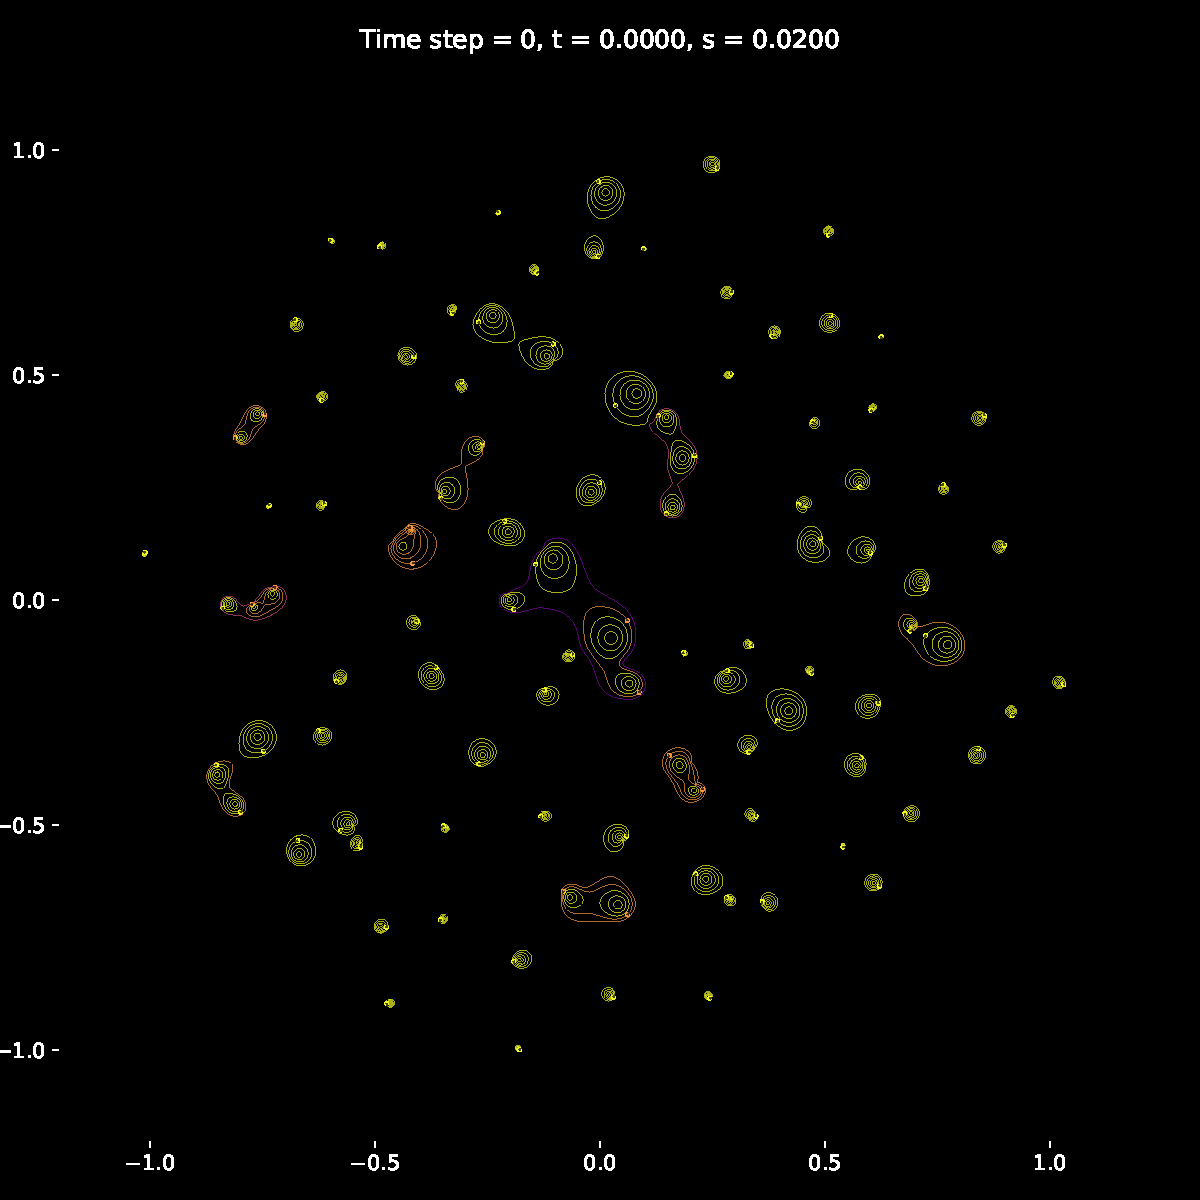
\includegraphics[width=0.8\textwidth]{/home/charli/Math/eigenvalueCollissions/animatedGinibre/frame0to50.pdf}
		\caption{Eigenvalue trajectories for $s= 0.005, 0.010, 0.015, 0.020, 0.025$ }
		\label{fig:pdf_image}
	\end{figure}


	\newpage

	\begin{figure}[htbp]
		\centering
		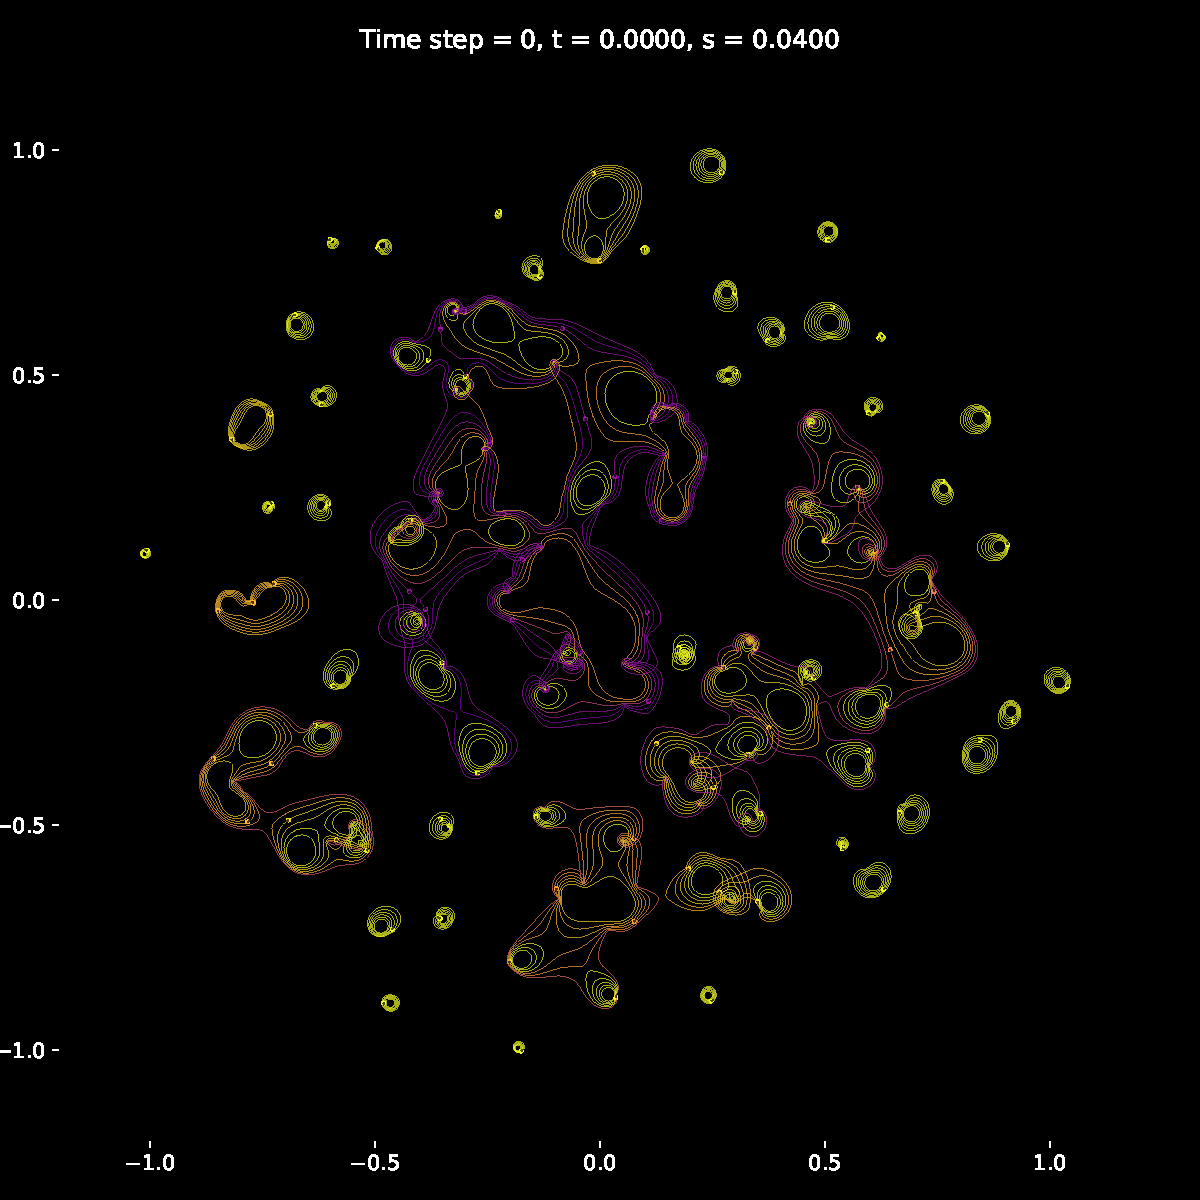
\includegraphics[width=0.8\textwidth]{/home/charli/Math/eigenvalueCollissions/animatedGinibre/frame50to100.pdf}
		\caption{Eigenvalue trajectories for $s= 0.025, 0.030, 0.035, 0.040, 0.045, 0.050$ }
		\label{fig:pdf_image}
	\end{figure}
	

\newpage

% \includegraphics[width=0.48\textwidth]{/home/charli/Math/eigenvalueTracking/animatedGinibre/frame95.pdf}

\begin{figure}[htbp]
    \centering
    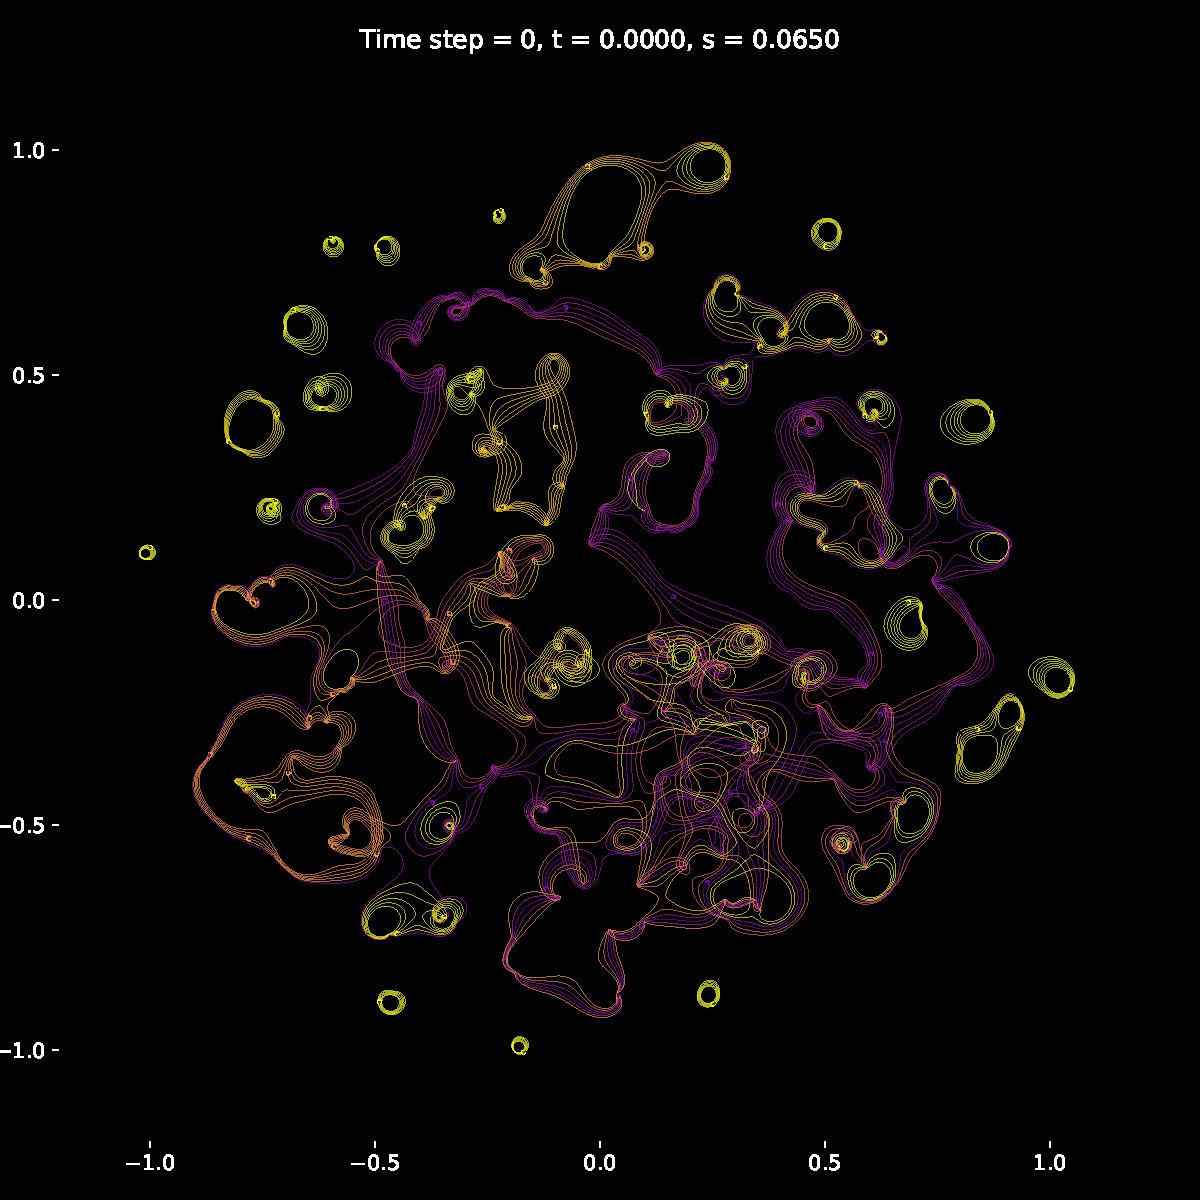
\includegraphics[width=0.8\textwidth]{/home/charli/Math/eigenvalueCollissions/animatedGinibre/frame100to150.pdf}
	\caption{Eigenvalue trajectories for $s= 0.050, 0.055, 0.060, 0.065, 0.070, 0.075$ }
    \label{fig:pdf_image}
\end{figure}


\newpage

% \includegraphics[width=0.48\textwidth]{/home/charli/Math/eigenvalueTracking/animatedGinibre/frame95.pdf}

\begin{figure}[htbp]
    \centering
    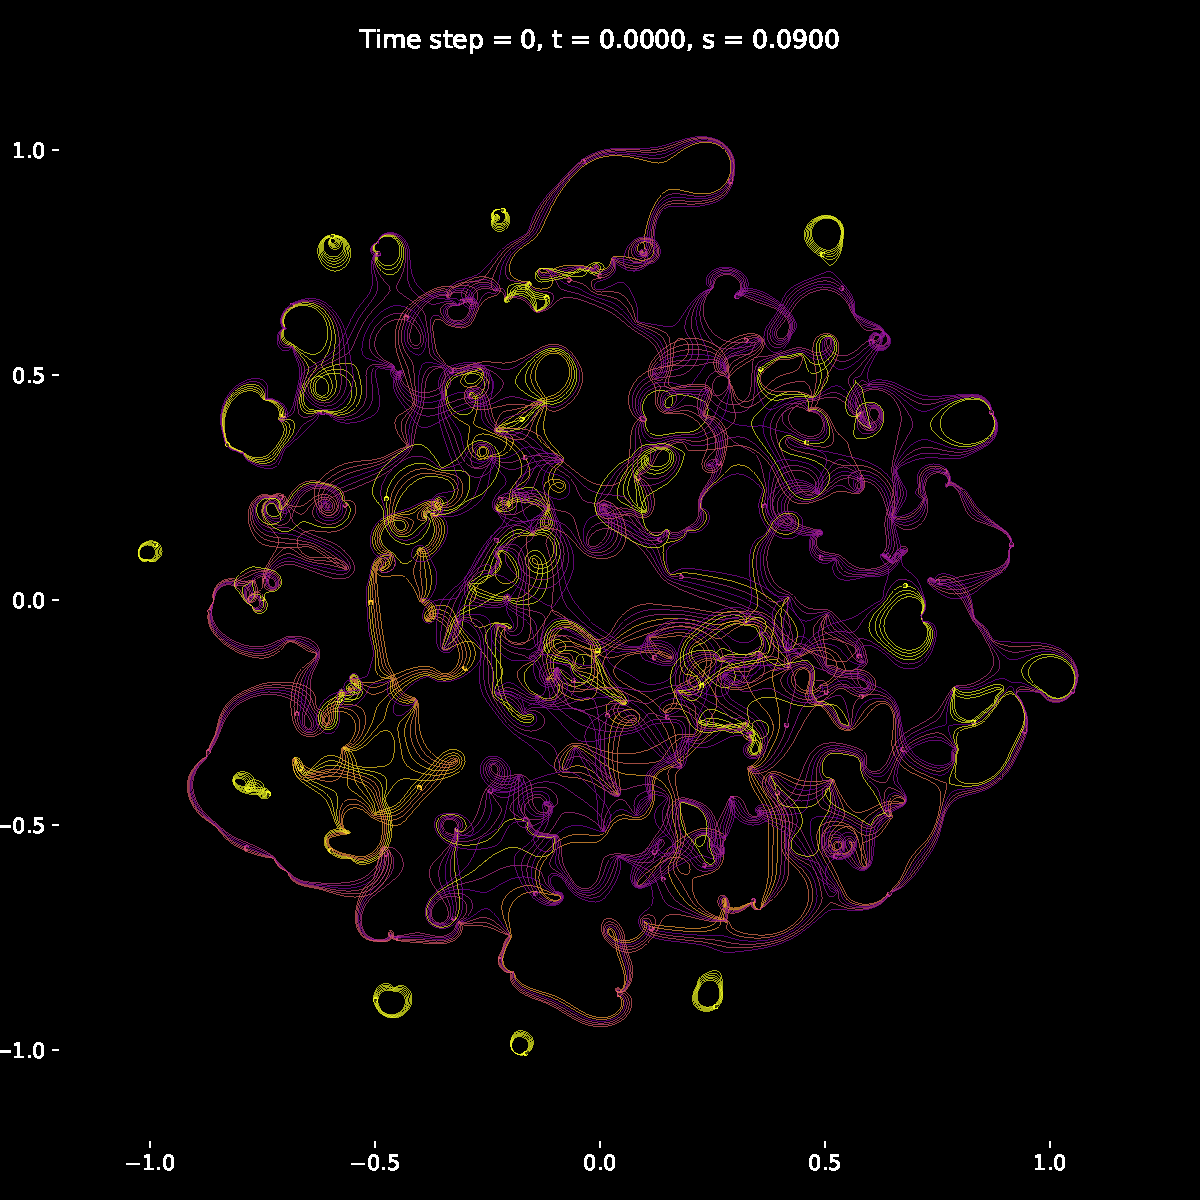
\includegraphics[width=0.8\textwidth]{/home/charli/Math/eigenvalueCollissions/animatedGinibre/frame150to200.pdf}
	\caption{Eigenvalue trajectories for $s= 0.075, 0.080, 0.085, 0.090, 0.095, 0.100$ }
    \label{fig:pdf_image}
\end{figure}


\newpage

% \includegraphics[width=0.48\textwidth]{/home/charli/Math/eigenvalueTracking/animatedGinibre/frame95.pdf}

\begin{figure}[htbp]
    \centering
    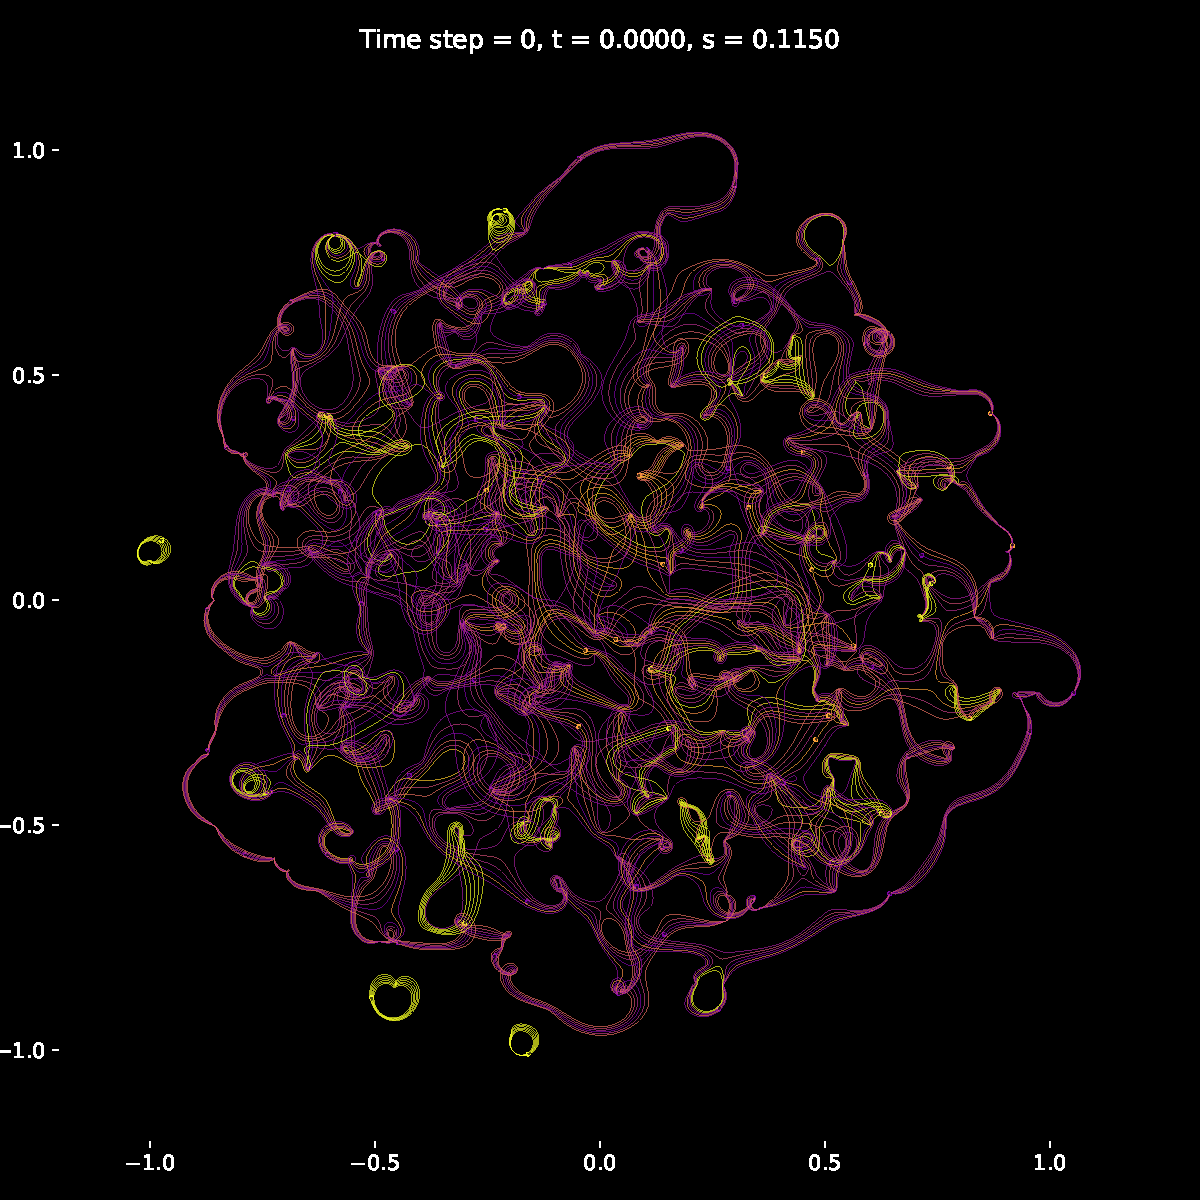
\includegraphics[width=0.8\textwidth]{/home/charli/Math/eigenvalueCollissions/animatedGinibre/frame200to250.pdf}
    \caption{Caption for your PDF image.}
    \label{fig:pdf_image}
\end{figure}


\newpage

% \includegraphics[width=0.48\textwidth]{/home/charli/Math/eigenvalueTracking/animatedGinibre/frame95.pdf}

\begin{figure}[htbp]
    \centering
    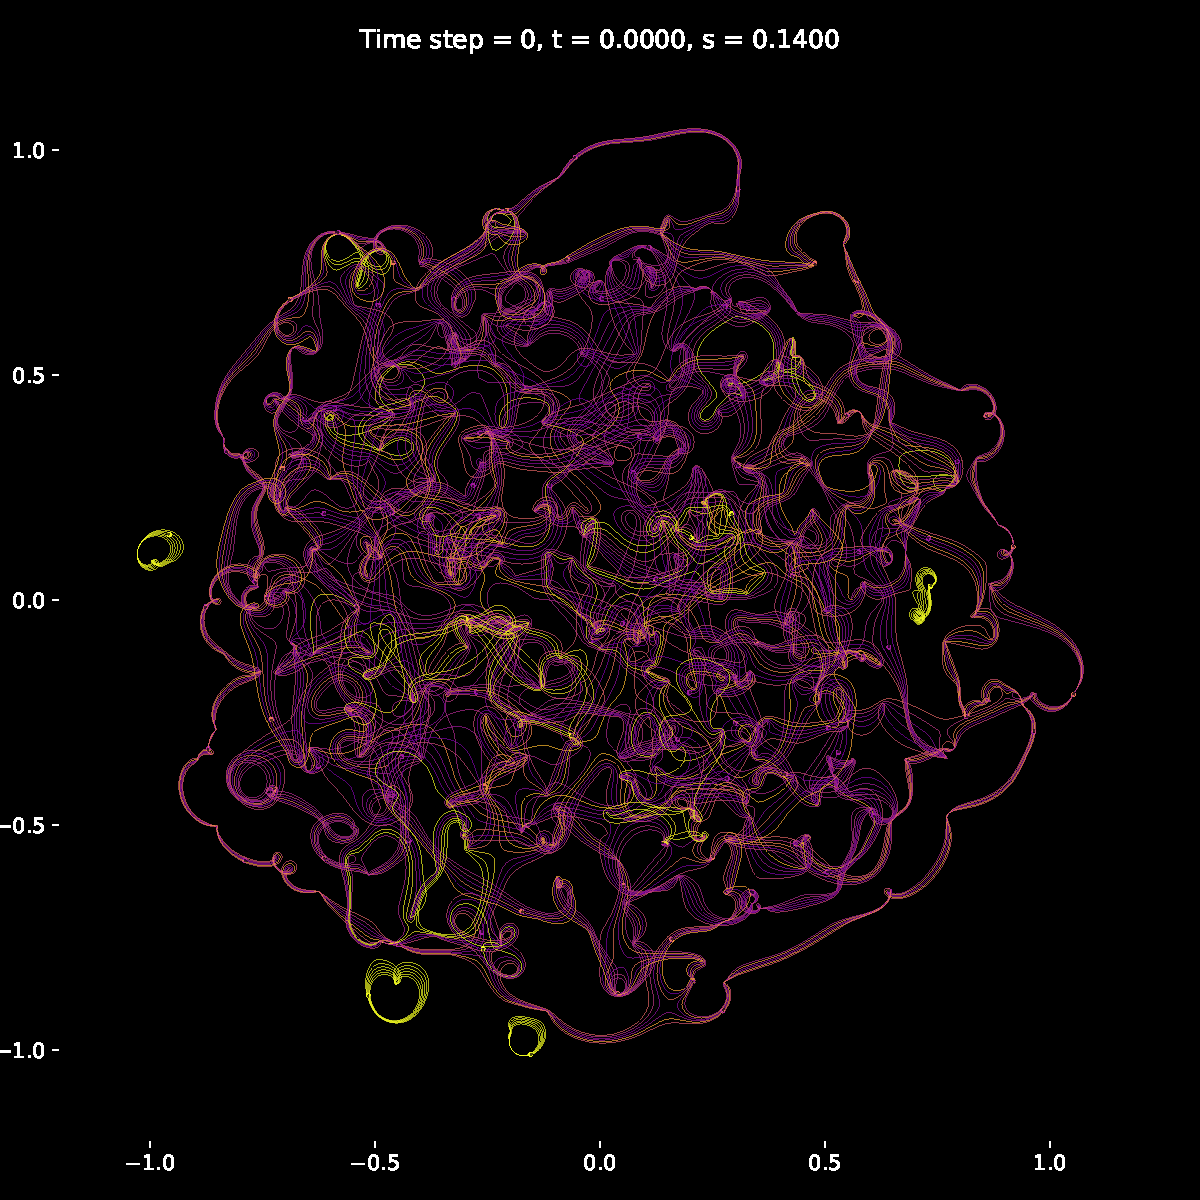
\includegraphics[width=0.8\textwidth]{/home/charli/Math/eigenvalueCollissions/animatedGinibre/frame250to300.pdf}
    \caption{Caption for your PDF image.}
    \label{fig:pdf_image}
\end{figure}

	In the next section we report some first statistics about these processes and their collisions.

	\section{Collision statistics}

	\section{About the algorithm}

	(TODO)
	General description of the algorithm. 
	
	Main bottleneck: linear algebraic library method for eigenvalues.
	Maybe a more specialized, explicitly pivoted method could 
	reduce computing time at this step.

	Counting algorithm vs exact solutions.

	Use of Delaunay Triangulations. 
	
	About condition number and shift.

	\section{Final Remarks}
	
	\section{References}

	- P. Zhong. (include reference...)
	

\end{document}